% ============================================================
% Cosmology history infographic — A4 landscape, LuaLaTeX
% Light editorial style: Libertinus Serif/Math + Hiragino,
% cream background, restrained palette, modern whitespace.
% Compile: lualatex cosmology-history.tex
% ============================================================
\documentclass[10pt]{article}
\usepackage[paperwidth=297mm, paperheight=210mm, margin=0pt]{geometry}
\usepackage{luatexja-fontspec}
\usepackage{tikz}
\usepackage{pgfplots}
\pgfplotsset{compat=1.18}
\usetikzlibrary{positioning, calc, shapes.geometric, shapes.misc, fadings,
  decorations.pathmorphing, backgrounds, fit, arrows.meta, patterns,
  shadings, matrix}
\usepackage{xcolor}
\usepackage{eso-pic}
\usepackage{unicode-math}

% ---- Fonts ----
\setmainfont{LibertinusSerif}[
  Extension      = .otf,
  UprightFont    = *-Regular,
  ItalicFont     = *-Italic,
  BoldFont       = *-Semibold,
  BoldItalicFont = *-SemiboldItalic,
  Numbers        = OldStyle,
]
\setsansfont{LibertinusSans}[
  Extension   = .otf,
  UprightFont = *-Regular,
  ItalicFont  = *-Italic,
  BoldFont    = *-Bold,
]
\setmathfont{LibertinusMath-Regular.otf}
\setmonofont{LibertinusMono-Regular.otf}

% Japanese: Hiragino on macOS. Mincho for body (refined), Sans for emphasis.
\setmainjfont{HiraMinProN-W3}[BoldFont=HiraMinProN-W6]
\setsansjfont{HiraginoSans-W3}[BoldFont=HiraginoSans-W6]

% ---- Palette: warm-to-cool temperature gradient, MUTED for light bg ----
\definecolor{c0}{HTML}{C73E3A}   % 1 inflation - deep red
\definecolor{c1}{HTML}{D2693C}   % 2 QGP       - rust orange
\definecolor{c2}{HTML}{C2942B}   % 3 BBN       - goldenrod
\definecolor{c3}{HTML}{6F8E2F}   % 4 M-R equal - olive
\definecolor{c4}{HTML}{2E8B8B}   % 5 recomb    - teal
\definecolor{c5}{HTML}{3865A1}   % 6 stars     - cobalt
\definecolor{c6}{HTML}{6B4F9E}   % 7 DE        - amethyst
\definecolor{c7}{HTML}{8E3D7E}   % 8 today     - magenta

\definecolor{plotrad}{HTML}{C73E3A}
\definecolor{plotmat}{HTML}{2E8B8B}
\definecolor{plotde}{HTML}{6B4F9E}

\definecolor{nucp}{HTML}{C73E3A}
\definecolor{nucn}{HTML}{3865A1}

% ---- Light theme surface tokens ----
\definecolor{bgpage}{HTML}{FBF8F2}     % cream paper
\definecolor{bgcard}{HTML}{FFFFFF}     % white card
\definecolor{bgcardb}{HTML}{E5E0D5}    % warm hairline
\definecolor{bgalt}{HTML}{F4EFE5}      % subtle alternate
\definecolor{fgstrong}{HTML}{1A1D26}   % near-black charcoal
\definecolor{fg}{HTML}{2E323F}
\definecolor{fgmute}{HTML}{6E7280}
\definecolor{fgfaint}{HTML}{A8A89E}
\definecolor{grid}{HTML}{E8E3D6}

% Background fill (= cream paper)
\AddToShipoutPictureBG*{\AtPageLowerLeft{\color{bgpage}\rule{\paperwidth}{\paperheight}}}

\pagestyle{empty}
\parindent=0pt

% ---- TikZ styles ----
\tikzset{
  card/.style={
    draw=bgcardb, line width=0.25pt,
    fill=bgcard,
    inner sep=0pt, outer sep=0pt,
  },
  stagenum/.style={
    circle, draw=none, fill=#1, text=white,
    font=\sffamily\bfseries\footnotesize,
    inner sep=0pt, minimum size=4mm,
  },
  proton/.style={circle, fill=nucp, inner sep=0pt, minimum size=#1},
  neutron/.style={circle, fill=nucn, inner sep=0pt, minimum size=#1},
}

% ---- Data row helper (in card-local coords) ----
\newcommand{\datarow}[3]{%
  \node[anchor=base west, font=\fontsize{6}{7}\selectfont\sffamily, text=fgmute, inner sep=0pt] at (-14, #1) {#2};%
  \node[anchor=base west, font=\fontsize{7}{8.5}\selectfont, text=fgstrong, inner sep=0pt] at (-9, #1) {#3};%
}

% ---- Icon macros (= simpler, more refined for light bg) ----
\newcommand{\iconInflation}[1]{%
  \begin{scope}[shift={(#1)}]
    \shade[inner color=c0!90!white, outer color=c0!20!white, opacity=0.85] (0,0) circle (3.5mm);
    \foreach \a in {0,45,...,315} {
      \draw[c0, line width=0.4pt, line cap=round] (\a:2mm) -- (\a:4.2mm);
    }
  \end{scope}
}
\newcommand{\iconQGP}[1]{%
  \begin{scope}[shift={(#1)}]
    \draw[c1!50!white, dashed, line width=0.25pt] (-2mm,-1mm) .. controls (0,0) .. (2mm,-1mm);
    \draw[c1!50!white, dashed, line width=0.25pt] (-2mm,1mm) .. controls (0,0) .. (2mm,1mm);
    \draw[c1!50!white, dashed, line width=0.25pt] (0,-2mm) .. controls (0,0) .. (0,2mm);
    \node[circle, fill=nucp, inner sep=0pt, minimum size=2.4mm,
          font=\fontsize{4}{4}\selectfont\sffamily\bfseries, text=white] at (-2mm,-1mm) {u};
    \node[circle, fill=nucp, inner sep=0pt, minimum size=2.4mm,
          font=\fontsize{4}{4}\selectfont\sffamily\bfseries, text=white] at (2mm,-1mm) {u};
    \node[circle, fill=nucn, inner sep=0pt, minimum size=2.4mm,
          font=\fontsize{4}{4}\selectfont\sffamily\bfseries, text=white] at (0,2mm) {d};
    \draw[c1!40!white, dashed, line width=0.25pt] (0,0) circle (3.2mm);
  \end{scope}
}
\newcommand{\nucleus}[3]{%
  \begin{scope}[shift={(#1)}]
    #3
    \node[font=\fontsize{4.5}{5}\selectfont, text=fg, anchor=north] at (0,-1.8mm) {#2};
  \end{scope}}
\newcommand{\iconBBN}[1]{%
  \begin{scope}[shift={(#1)}]
    \nucleus{-3.5mm,2mm}{$^{2}$H (D)}{%
      \node[proton=1.2mm] at (-0.7mm,0) {};
      \node[neutron=1.2mm] at (0.7mm,0) {};}
    \nucleus{3.5mm,2mm}{$^{3}$He}{%
      \node[proton=1.2mm] at (-0.8mm,-0.5mm) {};
      \node[proton=1.2mm] at (0.8mm,-0.5mm) {};
      \node[neutron=1.2mm] at (0,0.9mm) {};}
    \nucleus{-3.5mm,-2.5mm}{$^{4}$He}{%
      \node[proton=1.2mm] at (-0.8mm,-0.7mm) {};
      \node[proton=1.2mm] at (0.8mm,-0.7mm) {};
      \node[neutron=1.2mm] at (-0.8mm,0.7mm) {};
      \node[neutron=1.2mm] at (0.8mm,0.7mm) {};}
    \nucleus{3.5mm,-2.5mm}{$^{7}$Li}{%
      \node[proton=1mm] at (-1.1mm,-0.7mm) {};
      \node[proton=1mm] at (0,-1.2mm) {};
      \node[proton=1mm] at (1.1mm,-0.7mm) {};
      \node[neutron=1mm] at (-1.1mm,0.6mm) {};
      \node[neutron=1mm] at (0,1.2mm) {};
      \node[neutron=1mm] at (1.1mm,0.6mm) {};
      \node[neutron=1mm] at (0,0) {};}
  \end{scope}
}
\newcommand{\iconBalance}[1]{%
  \begin{scope}[shift={(#1)}]
    \draw[fg, line width=0.5pt] (0,-3mm) -- (0,3mm);
    \draw[fg, line width=0.5pt] (-4mm,3mm) -- (4mm,3mm);
    \begin{scope}[shift={(-3.5mm,1mm)}]
      \draw[fgmute, line width=0.2pt] (0,1.4mm) -- (-1mm,0);
      \draw[fgmute, line width=0.2pt] (0,1.4mm) -- (1mm,0);
      \draw[fg, line width=0.4pt, rounded corners=0.3mm] (-1.4mm,-0.4mm) rectangle (1.4mm,0.4mm);
      \draw[c2, line width=0.45pt] (-1mm,-1.4mm) .. controls (-0.5mm,-1mm) and (0,-1.8mm) .. (0.5mm,-1.4mm) .. controls (0.8mm,-1mm) and (1mm,-1.8mm) .. (1.2mm,-1.4mm);
    \end{scope}
    \begin{scope}[shift={(3.5mm,1mm)}]
      \draw[fgmute, line width=0.2pt] (0,1.4mm) -- (-1mm,0);
      \draw[fgmute, line width=0.2pt] (0,1.4mm) -- (1mm,0);
      \draw[fg, line width=0.4pt, rounded corners=0.3mm] (-1.4mm,-0.4mm) rectangle (1.4mm,0.4mm);
      \fill[plotmat] (-0.7mm,-1.2mm) circle (0.3mm);
      \fill[plotmat] (0,-1.2mm) circle (0.3mm);
      \fill[plotmat] (0.7mm,-1.2mm) circle (0.3mm);
    \end{scope}
    \fill[fg] (0,-3mm) -- (-0.8mm,-4.2mm) -- (0.8mm,-4.2mm) -- cycle;
  \end{scope}
}
\newcommand{\iconRecomb}[1]{%
  \begin{scope}[shift={(#1)}]
    \node[circle, fill=nucp, inner sep=0pt, minimum size=2.6mm,
          font=\fontsize{4}{4}\selectfont\sffamily\bfseries, text=white] at (-1.4mm,0) {p};
    \node[circle, fill=c6!75!white, inner sep=0pt, minimum size=1.6mm] at (1.4mm,0) {};
    \node[font=\fontsize{3.5}{3.5}\selectfont, text=fgmute] at (1.4mm,1.4mm) {e\textsuperscript{$-$}};
    \foreach \ang in {30,150,210,330}{
      \draw[plotmat, line width=0.4pt] (\ang:3.5mm) .. controls +(\ang+45:0.5mm) and +(\ang-45:0.5mm) .. (\ang:4.5mm);
    }
    \draw[plotmat!50!white, line width=0.2pt, dashed] (0,0) circle (3mm);
  \end{scope}
}
\newcommand{\iconStars}[1]{%
  \begin{scope}[shift={(#1)}]
    \foreach \p in {(-4mm,3mm),(4mm,3.5mm),(-4mm,-2.5mm),(3.5mm,-3mm),(0,4mm)}{
      \fill[fgmute] \p circle (0.18mm);
    }
    \shade[inner color=white, outer color=c5!80!white, opacity=0.95] (0,0) circle (1mm);
    \foreach \a in {0,45,...,315}{
      \draw[c5, line width=0.4pt, line cap=round] (\a:1.5mm) -- (\a:2.8mm);
    }
    \draw[plotmat!50!white, dashed, line width=0.2pt] (0,0) circle (4mm);
  \end{scope}
}
\newcommand{\iconDE}[1]{%
  \begin{scope}[shift={(#1)}]
    \fill[c6!80!white] (0,0) circle (1mm);
    \foreach \a in {90,210,330}{
      \draw[->, c6, line width=0.7pt, line cap=round, >={Stealth[length=1mm,width=1mm]}]
        (\a:1.5mm) -- (\a:4mm);
    }
    \foreach \a in {30,150,270}{
      \draw[c6!50!white, line width=0.3pt, line cap=round] (\a:1.7mm) -- (\a:3mm);
    }
  \end{scope}
}
\newcommand{\iconGalaxy}[1]{%
  \begin{scope}[shift={(#1)}]
    \foreach \p in {(-4mm,3mm),(4mm,3.5mm),(-4.5mm,-2.5mm),(4mm,-3mm),(-2mm,4mm),(2.5mm,-4mm),(5mm,1mm)}{
      \fill[fgmute] \p circle (0.18mm);
    }
    \begin{scope}[rotate=20]
      \draw[c5, line width=0.3pt, opacity=0.5] (0,0) ellipse (3.5mm and 1.4mm);
      \draw[c5, line width=0.5pt, opacity=0.8] (0,0) ellipse (2.8mm and 1.1mm);
      \fill[c5!40!white, opacity=0.4] (0,0) ellipse (2mm and 0.7mm);
      \fill[c2] (0,0) circle (0.6mm);
    \end{scope}
  \end{scope}
}

\begin{document}
\noindent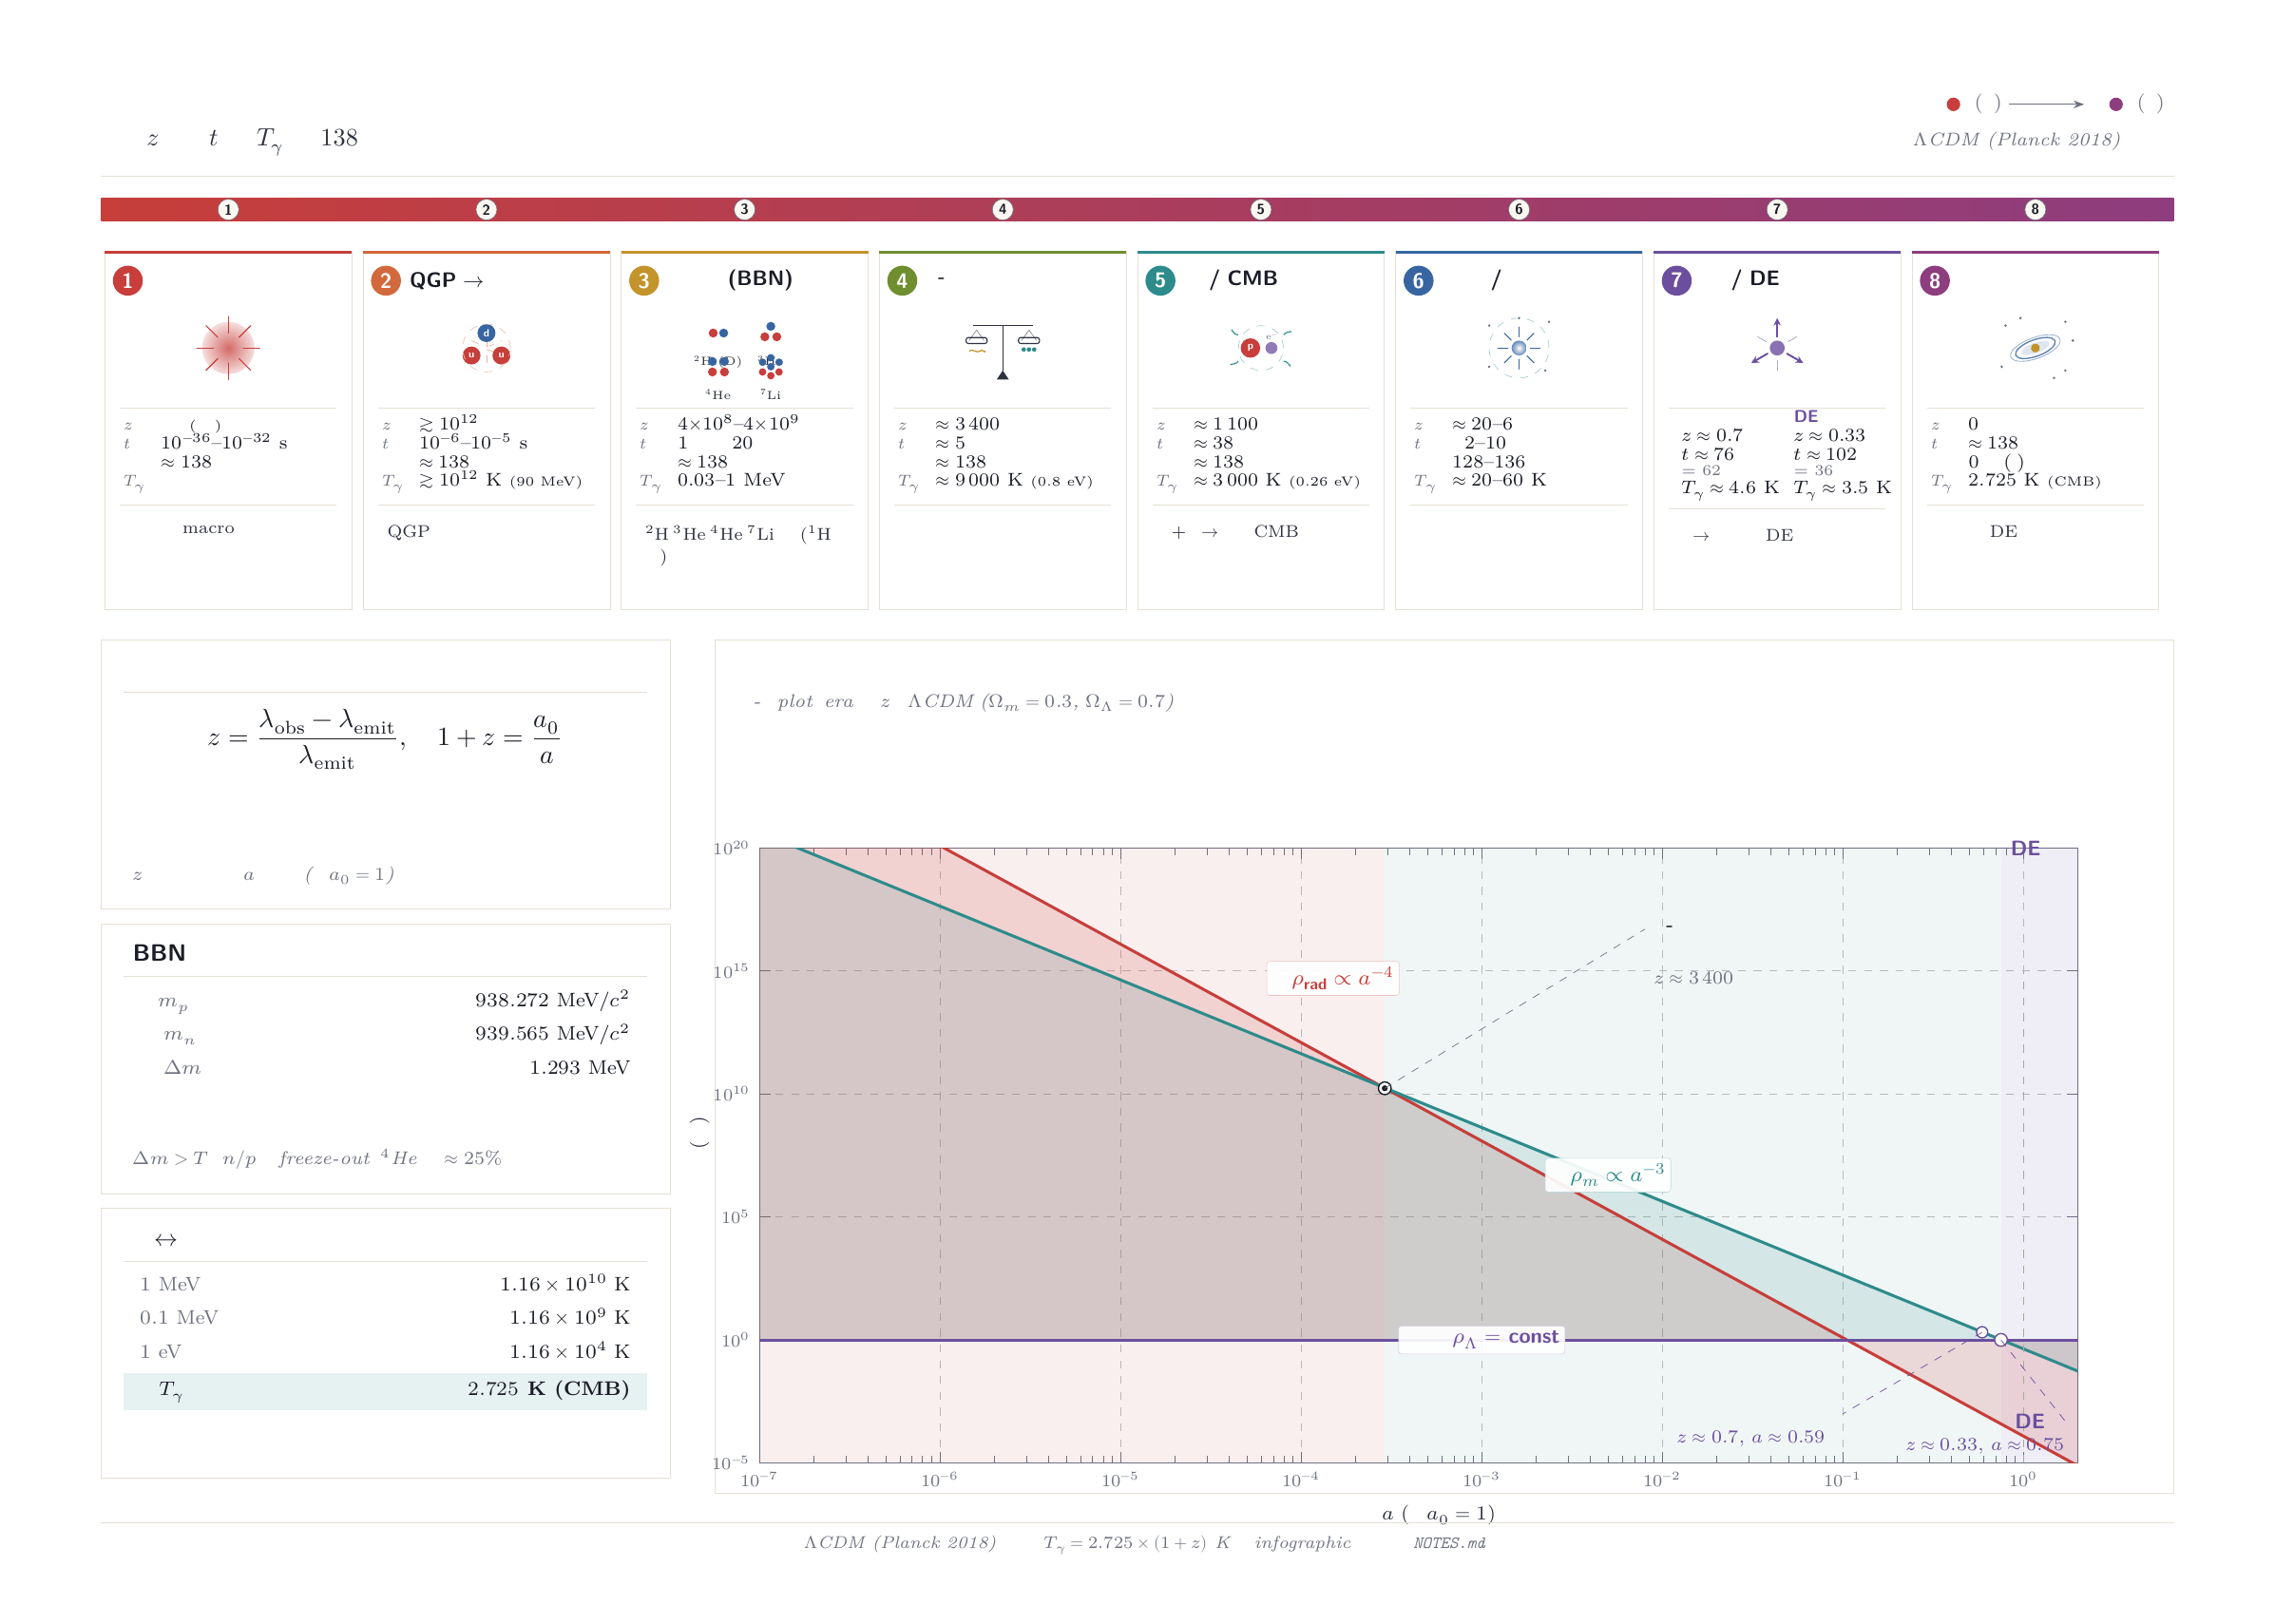
\begin{tikzpicture}[x=1mm, y=1mm]
  \useasboundingbox (0,0) rectangle (297, 210);

  % ====================== HEADER ======================
  \node[anchor=base west, font=\fontsize{28}{32}\selectfont\bfseries, text=fgstrong]
    at (10, 200) {宇宙の歴史};
  \node[anchor=base west, font=\fontsize{9.5}{11}\selectfont, text=fg]
    at (10, 194) {赤方偏移 $z$ ・宇宙年齢 $t$ ・温度 $T_{\gamma}$ で読む 138 億年};

  % Right-side: axis legend (= no boxed bg, just inline text)
  \node[anchor=base east, font=\fontsize{7.5}{9}\selectfont, text=fgmute]
    at (287, 199) {%
      \tikz[baseline=-0.5ex]{\fill[c0] (0,0) circle (0.9mm);}\,高温(初期)
      \tikz[baseline=-0.5ex]{\draw[fgmute, line width=0.25pt, ->, >={Stealth[length=1.4mm]}] (0,0) -- (10mm,0);} 時間
      \tikz[baseline=-0.5ex]{\fill[c7] (0,0) circle (0.9mm);}\,低温(現在)%
  };
  \node[anchor=base east, font=\fontsize{7}{8}\selectfont\itshape, text=fgmute]
    at (287, 194) {標準 $\Lambda$CDM (Planck 2018) に基づく代表値};

  % Header rule (hairline)
  \draw[bgcardb, line width=0.25pt] (10, 190) -- (287, 190);

  % ====================== HERO BAND (= thin temperature gradient) ======================
  \shade[left color=c0, right color=c7] (10, 184) rectangle (287, 187);
  \foreach \i/\x in {1/27, 2/61.5, 3/96, 4/130.5, 5/165, 6/199.5, 7/234, 8/268.5} {
    \node[circle, fill=bgpage, draw=fgmute, line width=0.2pt,
          font=\fontsize{5.5}{6}\selectfont\sffamily\bfseries, text=fgstrong,
          inner sep=0pt, minimum size=2.8mm] at (\x, 185.5) {\i};
  }

  % ====================== TIMELINE: 8 STAGE CARDS (48mm tall) ======================
  % Card y center = 156, top = 180, bottom = 132. Card width = 33mm.
  % Card x centers = 27, 61.5, 96, 130.5, 165, 199.5, 234, 268.5 (= 34.5mm apart, 1.5mm gap)
  \newcommand{\cardYmid}{156}

  % Internal coord (card-local origin = card center):
  %   y= 24 (top)   -- header
  %   y= 20         -- title baseline
  %   y= 14         -- icon center
  %   y=  4         -- separator
  %   y=  1, -1.5, -4, -6.5  -- 4 data rows
  %   y= -8.5       -- separator
  %   y= -10 down   -- description
  %   y=-24 (bottom)

  % ---------- Card 1 ----------
  \begin{scope}[shift={(27, \cardYmid)}]
    \node[card, minimum width=33mm, minimum height=48mm] at (0,0) {};
    \fill[c0] (-16.5,23.6) rectangle (16.5,24);  % top accent bar
    \node[stagenum=c0, anchor=west] at (-15.5, 20) {1};
    \node[anchor=west, font=\fontsize{8}{10}\selectfont\sffamily\bfseries, text=fgstrong,
          text width=22mm] at (-11.5, 20) {インフレーション};
    \iconInflation{0,11}
    \draw[bgcardb, line width=0.2pt] (-14.5, 3) -- (14.5, 3);
    \datarow{0}{$z$}{非常に大 \tiny(モデル依存)}
    \datarow{-2.5}{$t$}{$10^{-36}$--$10^{-32}$ s}
    \datarow{-5}{過去}{$\approx 138$ 億年前}
    \datarow{-7.5}{$T_{\gamma}$}{超高温}
    \draw[bgcardb, line width=0.2pt] (-14.5, -10) -- (14.5, -10);
    \node[anchor=north west, font=\fontsize{6.5}{8.5}\selectfont, text=fg,
          align=left, text width=29mm] at (-14.5, -11.5)
      {急膨張で量子ゆらぎが macro 化、 構造形成の種に。};
  \end{scope}

  % ---------- Card 2 ----------
  \begin{scope}[shift={(61.5, \cardYmid)}]
    \node[card, minimum width=33mm, minimum height=48mm] at (0,0) {};
    \fill[c1] (-16.5,23.6) rectangle (16.5,24);
    \node[stagenum=c1, anchor=west] at (-15.5, 20) {2};
    \node[anchor=west, font=\fontsize{8}{10}\selectfont\sffamily\bfseries, text=fgstrong,
          text width=22mm] at (-11.5, 20) {QGP $\to$ ハドロン化};
    \iconQGP{0,11}
    \draw[bgcardb, line width=0.2pt] (-14.5, 3) -- (14.5, 3);
    \datarow{0}{$z$}{$\gtrsim 10^{12}$}
    \datarow{-2.5}{$t$}{$10^{-6}$--$10^{-5}$ s}
    \datarow{-5}{過去}{$\approx 138$ 億年前}
    \datarow{-7.5}{$T_{\gamma}$}{$\gtrsim 10^{12}$ K \tiny(90 MeV)}
    \draw[bgcardb, line width=0.2pt] (-14.5, -10) -- (14.5, -10);
    \node[anchor=north west, font=\fontsize{6.5}{8.5}\selectfont, text=fg,
          align=left, text width=29mm] at (-14.5, -11.5)
      {QGP が冷えてハドロン化、 陽子・中性子に閉じ込め。};
  \end{scope}

  % ---------- Card 3 ----------
  \begin{scope}[shift={(96, \cardYmid)}]
    \node[card, minimum width=33mm, minimum height=48mm] at (0,0) {};
    \fill[c2] (-16.5,23.6) rectangle (16.5,24);
    \node[stagenum=c2, anchor=west] at (-15.5, 20) {3};
    \node[anchor=west, font=\fontsize{8}{10}\selectfont\sffamily\bfseries, text=fgstrong,
          text width=22mm] at (-11.5, 20) {ビッグバン元素合成 (BBN)};
    \iconBBN{0,11}
    \draw[bgcardb, line width=0.2pt] (-14.5, 3) -- (14.5, 3);
    \datarow{0}{$z$}{$4{\times}10^{8}$--$4{\times}10^{9}$}
    \datarow{-2.5}{$t$}{1 秒 〜 約 20 分}
    \datarow{-5}{過去}{$\approx 138$ 億年前}
    \datarow{-7.5}{$T_{\gamma}$}{$0.03$--$1$ MeV}
    \draw[bgcardb, line width=0.2pt] (-14.5, -10) -- (14.5, -10);
    \node[anchor=north west, font=\fontsize{6.5}{8.5}\selectfont, text=fg,
          align=left, text width=29mm] at (-14.5, -11.5)
      {$^{2}$H・$^{3}$He・$^{4}$He・$^{7}$Li が合成 ($^{1}$H は既存)。};
  \end{scope}

  % ---------- Card 4 ----------
  \begin{scope}[shift={(130.5, \cardYmid)}]
    \node[card, minimum width=33mm, minimum height=48mm] at (0,0) {};
    \fill[c3] (-16.5,23.6) rectangle (16.5,24);
    \node[stagenum=c3, anchor=west] at (-15.5, 20) {4};
    \node[anchor=west, font=\fontsize{8}{10}\selectfont\sffamily\bfseries, text=fgstrong,
          text width=22mm] at (-11.5, 20) {物質-放射等価};
    \iconBalance{0,11}
    \draw[bgcardb, line width=0.2pt] (-14.5, 3) -- (14.5, 3);
    \datarow{0}{$z$}{$\approx 3\,400$}
    \datarow{-2.5}{$t$}{$\approx 5$ 万年}
    \datarow{-5}{過去}{$\approx 138$ 億年前}
    \datarow{-7.5}{$T_{\gamma}$}{$\approx 9\,000$ K \tiny(0.8 eV)}
    \draw[bgcardb, line width=0.2pt] (-14.5, -10) -- (14.5, -10);
    \node[anchor=north west, font=\fontsize{6.5}{8.5}\selectfont, text=fg,
          align=left, text width=29mm] at (-14.5, -11.5)
      {放射と物質のエネルギー密度が等しく、 以後 物質優勢へ。};
  \end{scope}

  % ---------- Card 5 ----------
  \begin{scope}[shift={(165, \cardYmid)}]
    \node[card, minimum width=33mm, minimum height=48mm] at (0,0) {};
    \fill[c4] (-16.5,23.6) rectangle (16.5,24);
    \node[stagenum=c4, anchor=west] at (-15.5, 20) {5};
    \node[anchor=west, font=\fontsize{8}{10}\selectfont\sffamily\bfseries, text=fgstrong,
          text width=22mm] at (-11.5, 20) {再結合 / CMB 放射};
    \iconRecomb{0,11}
    \draw[bgcardb, line width=0.2pt] (-14.5, 3) -- (14.5, 3);
    \datarow{0}{$z$}{$\approx 1\,100$}
    \datarow{-2.5}{$t$}{$\approx 38$ 万年}
    \datarow{-5}{過去}{$\approx 138$ 億年前}
    \datarow{-7.5}{$T_{\gamma}$}{$\approx 3\,000$ K \tiny(0.26 eV)}
    \draw[bgcardb, line width=0.2pt] (-14.5, -10) -- (14.5, -10);
    \node[anchor=north west, font=\fontsize{6.5}{8.5}\selectfont, text=fg,
          align=left, text width=29mm] at (-14.5, -11.5)
      {電子+陽子 $\to$ 中性原子、 CMB が自由に伝播するように。};
  \end{scope}

  % ---------- Card 6 ----------
  \begin{scope}[shift={(199.5, \cardYmid)}]
    \node[card, minimum width=33mm, minimum height=48mm] at (0,0) {};
    \fill[c5] (-16.5,23.6) rectangle (16.5,24);
    \node[stagenum=c5, anchor=west] at (-15.5, 20) {6};
    \node[anchor=west, font=\fontsize{8}{10}\selectfont\sffamily\bfseries, text=fgstrong,
          text width=22mm] at (-11.5, 20) {最初の星・銀河 / 再電離};
    \iconStars{0,11}
    \draw[bgcardb, line width=0.2pt] (-14.5, 3) -- (14.5, 3);
    \datarow{0}{$z$}{$\approx 20$--$6$}
    \datarow{-2.5}{$t$}{約 2--10 億年}
    \datarow{-5}{過去}{128--136 億年前}
    \datarow{-7.5}{$T_{\gamma}$}{$\approx 20$--$60$ K}
    \draw[bgcardb, line width=0.2pt] (-14.5, -10) -- (14.5, -10);
    \node[anchor=north west, font=\fontsize{6.5}{8.5}\selectfont, text=fg,
          align=left, text width=29mm] at (-14.5, -11.5)
      {最初の星の{\bfseries 紫外光が中性ガスを再電離}。};
  \end{scope}

  % ---------- Card 7 (twocol) ----------
  \begin{scope}[shift={(234, \cardYmid)}]
    \node[card, minimum width=33mm, minimum height=48mm] at (0,0) {};
    \fill[c6] (-16.5,23.6) rectangle (16.5,24);
    \node[stagenum=c6, anchor=west] at (-15.5, 20) {7};
    \node[anchor=west, font=\fontsize{8}{10}\selectfont\sffamily\bfseries, text=fgstrong,
          text width=22mm] at (-11.5, 20) {加速膨張 / DE 優勢};
    \iconDE{0,11}
    \draw[bgcardb, line width=0.2pt] (-14.5, 3) -- (14.5, 3);
    % Two columns
    \node[anchor=base west, font=\fontsize{6.5}{8}\selectfont\sffamily\bfseries, text=c6] at (-14, 1) {加速開始};
    \node[anchor=base west, font=\fontsize{7}{8.5}\selectfont, text=fgstrong] at (-14, -1.5) {$z \approx 0.7$};
    \node[anchor=base west, font=\fontsize{7}{8.5}\selectfont, text=fgstrong] at (-14, -4) {$t \approx 76$ 億};
    \node[anchor=base west, font=\fontsize{5.8}{7}\selectfont, text=fgmute] at (-14, -6) {= 62 億年前};
    \node[anchor=base west, font=\fontsize{7}{8.5}\selectfont, text=fgstrong] at (-14, -8.5) {$T_{\gamma} \approx 4.6$ K};
    %
    \node[anchor=base west, font=\fontsize{6.5}{8}\selectfont\sffamily\bfseries, text=c6] at (1, 1) {DE 優勢};
    \node[anchor=base west, font=\fontsize{7}{8.5}\selectfont, text=fgstrong] at (1, -1.5) {$z \approx 0.33$};
    \node[anchor=base west, font=\fontsize{7}{8.5}\selectfont, text=fgstrong] at (1, -4) {$t \approx 102$ 億};
    \node[anchor=base west, font=\fontsize{5.8}{7}\selectfont, text=fgmute] at (1, -6) {= 36 億年前};
    \node[anchor=base west, font=\fontsize{7}{8.5}\selectfont, text=fgstrong] at (1, -8.5) {$T_{\gamma} \approx 3.5$ K};
    \draw[bgcardb, line width=0.2pt] (-14.5, -10.5) -- (14.5, -10.5);
    \node[anchor=north west, font=\fontsize{6.5}{8.5}\selectfont, text=fg,
          align=left, text width=29mm] at (-14.5, -12)
      {減速 $\to$ 加速膨張、 やがて DE が優勢に。};
  \end{scope}

  % ---------- Card 8 ----------
  \begin{scope}[shift={(268.5, \cardYmid)}]
    \node[card, minimum width=33mm, minimum height=48mm] at (0,0) {};
    \fill[c7] (-16.5,23.6) rectangle (16.5,24);
    \node[stagenum=c7, anchor=west] at (-15.5, 20) {8};
    \node[anchor=west, font=\fontsize{8}{10}\selectfont\sffamily\bfseries, text=fgstrong,
          text width=22mm] at (-11.5, 20) {現在};
    \iconGalaxy{0,11}
    \draw[bgcardb, line width=0.2pt] (-14.5, 3) -- (14.5, 3);
    \datarow{0}{$z$}{$0$}
    \datarow{-2.5}{$t$}{$\approx 138$ 億年}
    \datarow{-5}{過去}{0 年前 (今)}
    \datarow{-7.5}{$T_{\gamma}$}{$2.725$ K \tiny(CMB)}
    \draw[bgcardb, line width=0.2pt] (-14.5, -10) -- (14.5, -10);
    \node[anchor=north west, font=\fontsize{6.5}{8.5}\selectfont, text=fg,
          align=left, text width=29mm] at (-14.5, -11.5)
      {銀河・星・惑星のある DE 優勢の宇宙。};
  \end{scope}

  % ====================== BOTTOM ROW: info stack + plot ======================
  % Available y: 14 to 128 = 114mm tall, with 4mm internal gaps
  % Left (info): x=10 to 86 (76mm wide)
  % Right (plot): x=92 to 287 (195mm wide)

  % ----- Info card 1: redshift formula -----
  \begin{scope}[shift={(10, 128)}]
    \node[card, anchor=north west, minimum width=76mm, minimum height=36mm] at (0,0) {};
    \node[anchor=base west, font=\fontsize{9}{11}\selectfont\sffamily\bfseries, text=fgstrong]
      at (3, -5) {赤方偏移};
    \draw[bgcardb, line width=0.2pt] (3, -7) -- (73, -7);
    \node[anchor=north, font=\fontsize{10}{12}\selectfont, text=fgstrong]
      at (38, -8) {$\displaystyle z = \frac{\lambda_{\text{obs}} - \lambda_{\text{emit}}}{\lambda_{\text{emit}}}, \quad 1 + z = \frac{a_{0}}{a}$};
    \node[anchor=south west, font=\fontsize{7}{9}\selectfont\itshape, text=fgmute, text width=70mm]
      at (3, -34) {$z$ は過去ほど、 遠い宇宙ほど大きい。 $a$ はスケール因子 (現在 $a_{0} = 1$)。};
  \end{scope}

  % ----- Info card 2: BBN physics -----
  \begin{scope}[shift={(10, 90)}]
    \node[card, anchor=north west, minimum width=76mm, minimum height=36mm] at (0,0) {};
    \node[anchor=base west, font=\fontsize{9}{11}\selectfont\sffamily\bfseries, text=fgstrong]
      at (3, -5) {BBN の核物理メモ};
    \draw[bgcardb, line width=0.2pt] (3, -7) -- (73, -7);
    \node[anchor=base west, font=\fontsize{7.5}{9}\selectfont, text=fgmute] at (4, -11) {陽子 $m_{p}$};
    \node[anchor=base east, font=\fontsize{7.5}{9}\selectfont, text=fgstrong] at (72, -11) {$938.272$ MeV/$c^{2}$};
    \node[anchor=base west, font=\fontsize{7.5}{9}\selectfont, text=fgmute] at (4, -15.5) {中性子 $m_{n}$};
    \node[anchor=base east, font=\fontsize{7.5}{9}\selectfont, text=fgstrong] at (72, -15.5) {$939.565$ MeV/$c^{2}$};
    \node[anchor=base west, font=\fontsize{7.5}{9}\selectfont, text=fgmute] at (4, -20) {質量差 $\Delta m$};
    \node[anchor=base east, font=\fontsize{7.5}{9}\selectfont, text=fgstrong] at (72, -20) {$1.293$ MeV};
    \node[anchor=south west, font=\fontsize{7}{9}\selectfont\itshape, text=fgmute, text width=70mm]
      at (3, -34) {$\Delta m > T$ で $n/p$ 比が freeze-out、 $^{4}$He 質量比 $\approx 25\%$。};
  \end{scope}

  % ----- Info card 3: temperature conversions -----
  \begin{scope}[shift={(10, 52)}]
    \node[card, anchor=north west, minimum width=76mm, minimum height=36mm] at (0,0) {};
    \node[anchor=base west, font=\fontsize{9}{11}\selectfont\sffamily\bfseries, text=fgstrong]
      at (3, -5) {温度 $\leftrightarrow$ エネルギー};
    \draw[bgcardb, line width=0.2pt] (3, -7) -- (73, -7);
    \node[anchor=base west, font=\fontsize{7.5}{9}\selectfont, text=fgmute] at (4, -11) {$1$ MeV};
    \node[anchor=base east, font=\fontsize{7.5}{9}\selectfont, text=fgstrong] at (72, -11) {$1.16 \times 10^{10}$ K};
    \node[anchor=base west, font=\fontsize{7.5}{9}\selectfont, text=fgmute] at (4, -15.5) {$0.1$ MeV};
    \node[anchor=base east, font=\fontsize{7.5}{9}\selectfont, text=fgstrong] at (72, -15.5) {$1.16 \times 10^{9}$ K};
    \node[anchor=base west, font=\fontsize{7.5}{9}\selectfont, text=fgmute] at (4, -20) {$1$ eV};
    \node[anchor=base east, font=\fontsize{7.5}{9}\selectfont, text=fgstrong] at (72, -20) {$1.16 \times 10^{4}$ K};
    % highlight row
    \fill[c4!12!bgcard] (3, -27) rectangle (73, -22);
    \node[anchor=base west, font=\fontsize{7.5}{9}\selectfont\bfseries, text=fgstrong] at (4, -25) {現在 $T_{\gamma}$};
    \node[anchor=base east, font=\fontsize{7.5}{9}\selectfont\bfseries, text=fgstrong] at (72, -25) {$2.725$ K (CMB)};
  \end{scope}

  % ====================== DENSITY PLOT ======================
  % Plot card: x = 92 to 287 (width 195mm), y = 14 to 128 (height 114mm)
  \node[card, anchor=south west, minimum width=195mm, minimum height=114mm] at (92, 14) {};
  \node[anchor=base west, font=\fontsize{9.5}{12}\selectfont\sffamily\bfseries, text=fgstrong]
    at (94.5, 123) {宇宙の主要成分のエネルギー密度};
  \node[anchor=base west, font=\fontsize{7}{9}\selectfont\itshape, text=fgmute, text width=190mm]
    at (94.5, 119) {対数-対数 plot。 era 境界の $z$ は $\Lambda$CDM ($\Omega_{m} = 0.3$, $\Omega_{\Lambda} = 0.7$) より};

  \begin{scope}[shift={(98, 18)}]
    \begin{axis}[
      width=192mm, height=98mm,
      xmode=log, ymode=log,
      xmin=1e-7, xmax=2,
      ymin=1e-5, ymax=1e20,
      axis line style={fgmute, line width=0.3pt},
      tick style={fgmute, line width=0.3pt},
      tick label style={font=\fontsize{6.5}{8}\selectfont, text=fgmute},
      xlabel style={font=\fontsize{7.5}{9}\selectfont, text=fg},
      ylabel style={font=\fontsize{7.5}{9}\selectfont, text=fg, yshift=-2mm},
      xlabel={スケール因子 $a$ (現在 $a_{0} = 1$)},
      ylabel={エネルギー密度 (相対値)},
      xtick={1e-7, 1e-6, 1e-5, 1e-4, 1e-3, 1e-2, 1e-1, 1},
      ytick={1e-5, 1, 1e5, 1e10, 1e15, 1e20},
      grid=major,
      grid style={grid, line width=0.2pt, dashed},
      clip mode=individual,
      enlargelimits=false,
      every axis plot/.append style={line cap=round},
    ]

      % Era background bands
      \fill[plotrad, opacity=0.08] (axis cs:1e-7,1e-5) rectangle (axis cs:2.9e-4,1e20);
      \fill[plotmat, opacity=0.07] (axis cs:2.9e-4,1e-5) rectangle (axis cs:0.75,1e20);
      \fill[plotde,  opacity=0.10] (axis cs:0.75,1e-5)   rectangle (axis cs:2,1e20);

      % Area fills under lines
      \addplot[fill=plotrad, fill opacity=0.16, draw=none, domain=1e-7:2, samples=80]
        {1.22e-4 * x^(-4)} \closedcycle;
      \addplot[fill=plotmat, fill opacity=0.14, draw=none, domain=1e-7:2, samples=80]
        {0.43 * x^(-3)} \closedcycle;
      \addplot[fill=plotde, fill opacity=0.16, draw=none, domain=1e-7:2, samples=2]
        {1} \closedcycle;

      % Main lines
      \addplot[plotrad, line width=1.1pt, domain=1e-7:2, samples=80]
        {1.22e-4 * x^(-4)};
      \addplot[plotmat, line width=1.1pt, domain=1e-7:2, samples=80]
        {0.43 * x^(-3)};
      \addplot[plotde, line width=1.1pt, domain=1e-7:2, samples=2]
        {1};

      % Crossover markers
      \node[circle, fill=bgcard, draw=fgstrong, line width=0.5pt, inner sep=0pt, minimum size=1.7mm]
        at (axis cs:2.9e-4, 1.7e10) {};
      \node[circle, fill=fgstrong, inner sep=0pt, minimum size=0.8mm]
        at (axis cs:2.9e-4, 1.7e10) {};

      \node[circle, fill=bgcard, draw=plotde, line width=0.5pt, inner sep=0pt, minimum size=1.5mm]
        at (axis cs:0.59, 2.05) {};
      \node[circle, fill=bgcard, draw=plotde, line width=0.5pt, inner sep=0pt, minimum size=1.7mm]
        at (axis cs:0.75, 1) {};

      % "Now" marker at a=1
      \draw[fgfaint, dashed, line width=0.3pt] (axis cs:1, 1e-5) -- (axis cs:1, 1e15);
      \node[font=\fontsize{6.5}{7}\selectfont, text=fgmute, anchor=south] at (axis cs:1, 1e15) {現在};

      % Era labels above plot
      \node[font=\fontsize{8}{9}\selectfont\sffamily\bfseries, text=plotrad] at (axis cs:1e-5, 1e20) {放射優勢};
      \node[font=\fontsize{8}{9}\selectfont\sffamily\bfseries, text=plotmat] at (axis cs:1e-2, 1e20) {物質優勢};
      \node[font=\fontsize{8}{9}\selectfont\sffamily\bfseries, text=plotde,  anchor=east] at (axis cs:1.8, 1e20) {DE 優勢};

      % Direct in-plot line labels (= solid bg, slight border for crispness)
      \node[font=\fontsize{8}{10}\selectfont\sffamily\bfseries, text=plotrad,
            fill=bgcard, fill opacity=0.92, text opacity=1, inner sep=0.7mm, rounded corners=0.4mm,
            draw=plotrad!30!bgcard, line width=0.2pt]
        at (axis cs:1.5e-4, 5e14) {放射 $\rho_{\text{rad}} \propto a^{-4}$};
      \node[font=\fontsize{8}{10}\selectfont\sffamily\bfseries, text=plotmat,
            fill=bgcard, fill opacity=0.92, text opacity=1, inner sep=0.7mm, rounded corners=0.4mm,
            draw=plotmat!30!bgcard, line width=0.2pt]
        at (axis cs:5e-3, 5e6) {物質 $\rho_{m} \propto a^{-3}$};
      \node[font=\fontsize{8}{10}\selectfont\sffamily\bfseries, text=plotde,
            fill=bgcard, fill opacity=0.92, text opacity=1, inner sep=0.7mm, rounded corners=0.4mm,
            draw=plotde!30!bgcard, line width=0.2pt]
        at (axis cs:1e-3, 1) {暗黒エネルギー $\rho_{\Lambda} = $ const};

      % Annotations with leader lines
      \draw[fgmute, dashed, line width=0.25pt] (axis cs:2.9e-4, 1.7e10) -- (axis cs:8e-3, 5e16);
      \node[font=\fontsize{8}{10}\selectfont\sffamily\bfseries, text=fgstrong, anchor=west] at (axis cs:8e-3, 5e16) {物質-放射等価};
      \node[font=\fontsize{7}{9}\selectfont, text=fgmute, anchor=west] at (axis cs:8e-3, 5e14) {$z \approx 3\,400$};

      \draw[plotde, dashed, line width=0.25pt] (axis cs:0.59, 2.05) -- (axis cs:0.1, 1e-3);
      \node[font=\fontsize{8}{10}\selectfont\sffamily\bfseries, text=plotde, anchor=east] at (axis cs:0.09, 1e-3) {加速膨張開始};
      \node[font=\fontsize{7}{9}\selectfont, text=plotde, anchor=east] at (axis cs:0.09, 1e-4) {$z \approx 0.7$, $a \approx 0.59$};

      \draw[plotde, dashed, line width=0.25pt] (axis cs:0.75, 1) -- (axis cs:1.7, 5e-4);
      \node[font=\fontsize{8}{10}\selectfont\sffamily\bfseries, text=plotde, anchor=east] at (axis cs:1.9, 5e-4) {DE 優勢};
      \node[font=\fontsize{7}{9}\selectfont, text=plotde, anchor=east] at (axis cs:1.9, 5e-5) {$z \approx 0.33$, $a \approx 0.75$};

    \end{axis}
  \end{scope}

  % ====================== FOOTER ======================
  \draw[bgcardb, line width=0.2pt] (10, 10) -- (287, 10);
  \node[font=\fontsize{6.5}{8}\selectfont\itshape, text=fgmute, anchor=center] at (148.5, 7)
    {数値は標準 $\Lambda$CDM (Planck 2018) 代表値・近似。 $T_{\gamma} = 2.725 \times (1+z)$ K。 元 infographic からの修正点と典拠は \texttt{NOTES.md} 参照};

\end{tikzpicture}
\end{document}
